\chapter{Resultados e Discussão}

Nesta seção apresentamos os resultados obtidos a partir da análise das coautorias, onde são discutidos os resultados relacionados à produção bibliográfica, impacto e colaboração com as demais áreas e a interdisciplinaridade da Ciência da Computação, comparando-a com as demais áreas e discutindo como suas relações acontecem sob o ponto de vista das coautorias.

\section{Produção bibliográfica}

O número de publicações científicas únicas feitas em coautoria com pesquisadores da Ciência da Computação é de $282.796$, sendo a 5ª área que mais colabora considerando as publicações de todos os tempos, ficando atrás apenas da Medicina, Agronomia, Educação e Química, como mostra a \autoref{tab:producaoporarea}.

\begin{table}[htpb]
    \centering
    \caption{As 10 áreas que mais produzem publicações científicas em coautoria na ciência brasileira.}
    \label{tab:producaoporarea}
    \begin{tabular}{|r|l|c|}%
        \hline & Área & Número de publicações\\\hline
        \csvreader[late after line=\\\hline]%
        {"tabelas/resultados-producao-bliografica-por-area.csv"}%
        {area=\area,contagem=\contagem}%
        {\thecsvrow & \area & \contagem}%
    \end{tabular}
\end{table}

A \autoref{fig:coautoriaanual} apresenta um gráfico de segmento anual, que vai do ano de surgimento do Currículo Lattes até o último ano completo, com o crescimento do número de publicações feitas em coautoria das áreas que mais produzem em coautoria. Nele é possível observar que o crescimento do número de coautorias da Ciência da Computação não foi alto, e acompanhou as demais áreas do conhecimento consideradas.

São exceções as áreas de Educação e Medicina, que durante os períodos de 2004-2009 e 2002-2006, respectivamente, tiveram crescimento acelerado e depois se mantiveram estáveis. Ainda, é importante pontuar que existe uma queda acentuada em todas as áreas no ano de 2018, mas isso está provavelmente relacionado ao fato da coleta ter sido feita em janeiro de 2019 e as publicações do ano de 2018 não terem sido todas concluídas.

\begin{figure}[htpb]
  \centering
  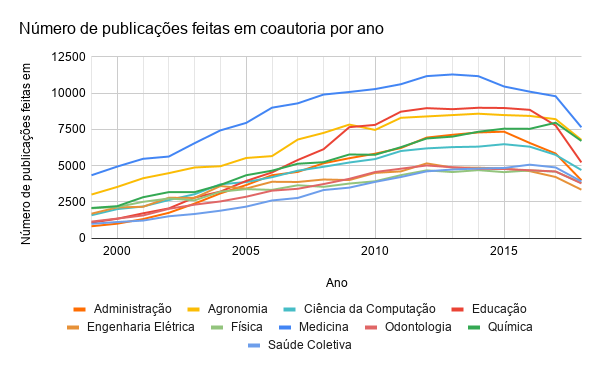
\includegraphics[width=1\textwidth]{figuras/resultados-grafico-coautoria-anual}
  \caption{Gráfico de segmento anual com a produção em coautoria das áreas que mais produzem em coautoria no período de 1999 a 2018.}
  \label{fig:coautoriaanual}
\end{figure}

\section{Impacto e colaboração}

A rede de colaboração entre as áreas apresentada na \autoref{fig:grafocolaboracao} foi construída a partir da rede de coautoria entre os pesquisadores. O diâmetro da rede é igual a $3$, o caminho médio igual a $1,31$ e coeficiente médio de clusterização igual a $0,912$. Essa rede apresenta um comportamento comumente observado em redes sociais, é coesa e se caracteriza pela alta densidade de arestas, indicando que quase todas as áreas do conhecimento estão relacionadas entre si. Este fato observado se comporta como o esperado, dado que na ciência não se trabalha de forma isolada.

\begin{figure}[htpb]
  \centering
  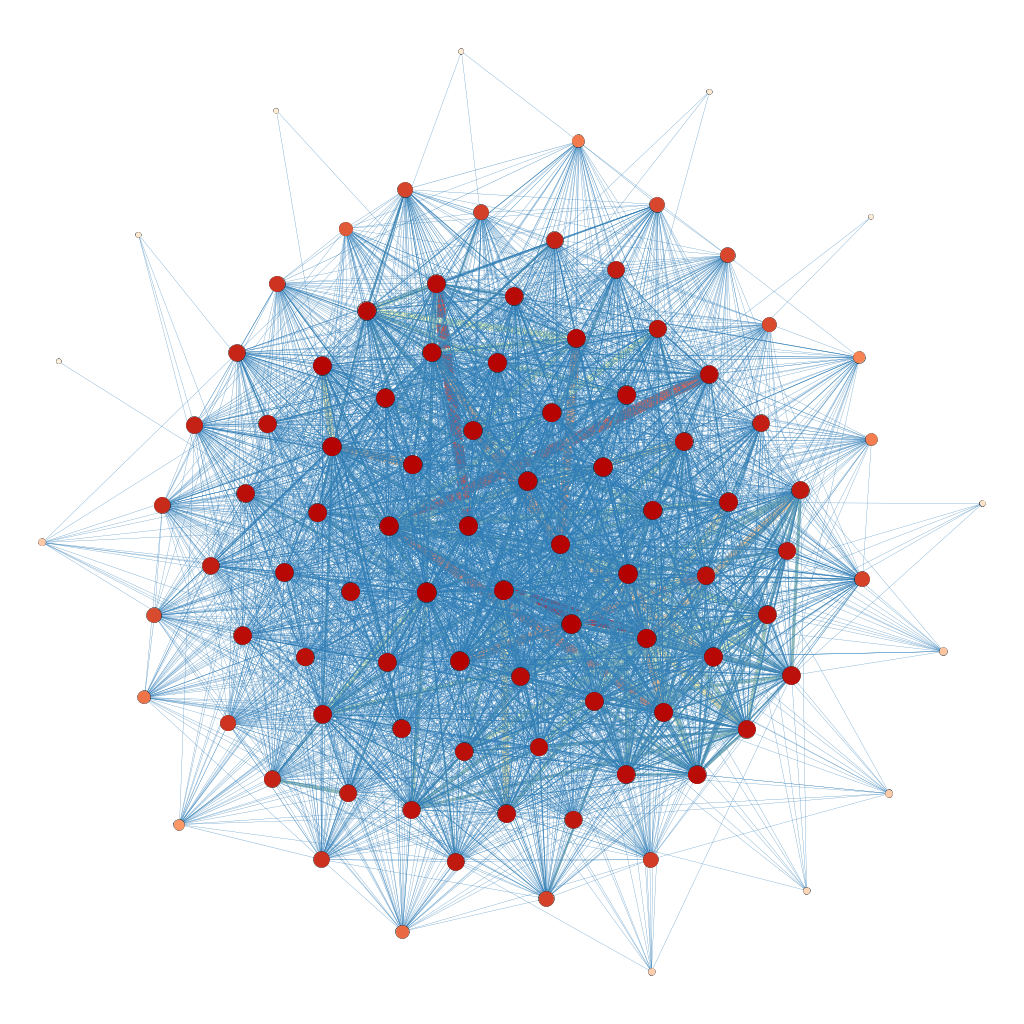
\includegraphics[width=1\textwidth]{figuras/resultados-grafo-colaboracao-entre-areas}
  \caption{Grafo de colaboração entre as áreas do conhecimento.}
  \label{fig:grafocolaboracao}
\end{figure}

O mapa de calor obtido na \autoref{fig:mapadecalorcolaboracao}, com a colaboração exercida entre as áreas, mostra que o maior esforço de colaboração da Ciência da Computação está com a Engenharia Elétrica, sendo que as áreas mais impactadas pela Ciência da Computação são a Matemática, Engenharia Elétrica e Ciência da Informação. Ainda segundo este mapa, podemos ver que a Medicina é a área que mais impacta áreas distintas.

\begin{landscape}
  \begin{figure}[htbp]
    \centering
    \includegraphics[width=\linewidth, height=\textheight, keepaspectratio]%
    {figuras/resultados-mapa-de-calor-colaboracao-entre-areas}
    \caption{Mapa de calor das colaborações exercidas entre as áreas. As linhas horizontais podem ser interpretadas como o impacto exercido e as linhas verticais podem ser entendidas como a relevância que outra área recebeu esse impacto.}
    \label{fig:mapadecalorcolaboracao}
  \end{figure}
\end{landscape}

Uma visualização que permite observar o impacto exercido por cada área é apresentada na \autoref{fig:grafoimpacto}, uma interpretação do mesmo mapa de calor, onde os nós são as áreas do conhecimento e as arestas direcionadas representam o impacto que é exercido pela área, isto é, quanto das suas colaborações determinam as produção científica feita em colaboração das outras áreas.

Nele é possível observar que existem $7$ componentes conexas, a maior componente conexa conta com 61 nós, o que representa $62,89$\% da rede. A Ciência da Computação faz parte de um subgrafo que está interconectado pela Engenharia da Computação, onde pode ser visto que de fato o impacto é relevante apenas na Engenharia Elétrica.

\begin{figure}[htpb]
  \centering
  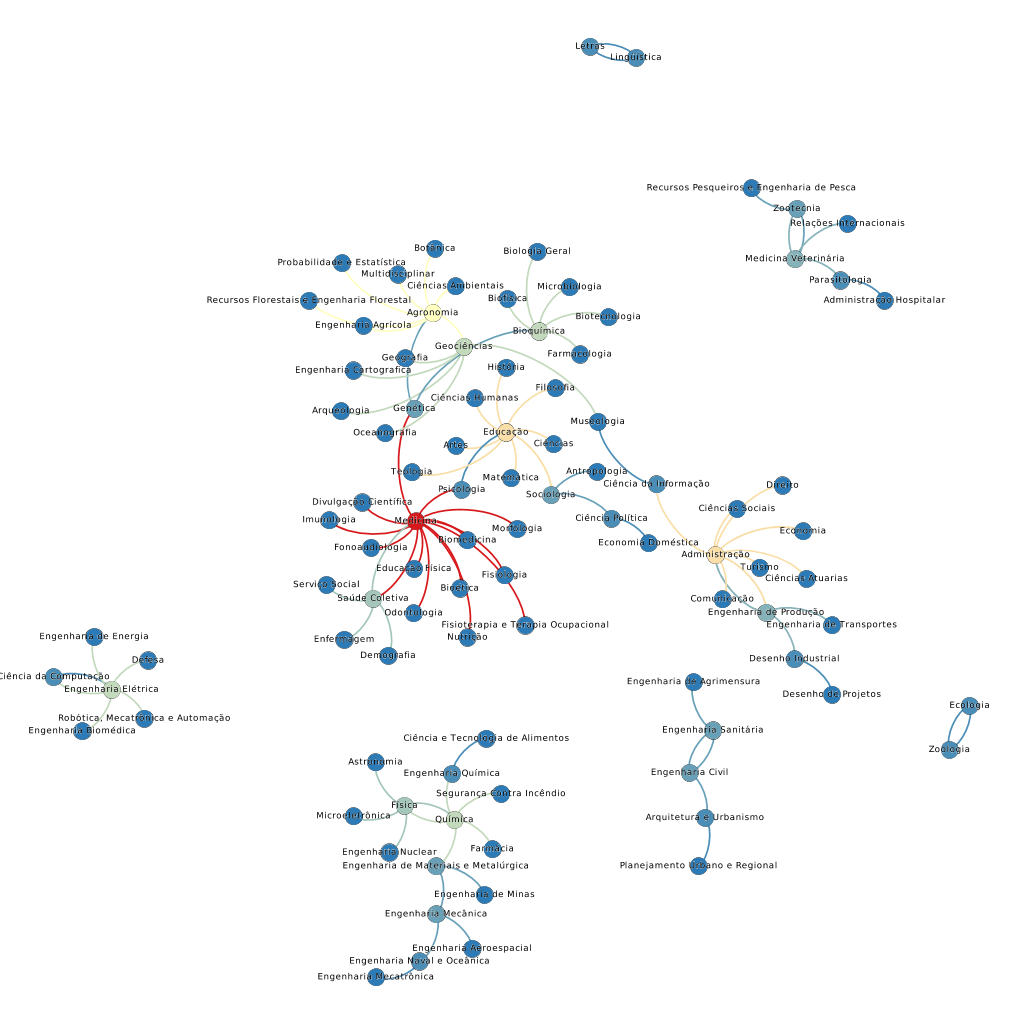
\includegraphics[width=1\textwidth]{figuras/resultados-grafo-impacto}
  \caption{Grafo do impacto exercido pela área na produção científica feita em colaboração das outras áreas. Os nós com cores mais quentes são os que mais exercem impacto em outras áreas.}
  \label{fig:grafoimpacto}
\end{figure}

\section{Interdisciplinaridade}

Interdisciplinaridade é um conceito que pode ser interpretado de diferentes maneiras. Neste trabalho uma publicação em coautoria será considerada interdisciplinar se os coautores pertencem a pelo menos 3 áreas distintas.

O número de publicações científicas interdisciplinares feitas em coautoria apresentado na \autoref{tab:producaointerdisciplinar} mostra que a Ciência da Computação, apesar de construir muitas publicações em coautoria, não tem muita atuação em projetos desse tipo.

\begin{table}[htpb]
    \centering
    \caption{As 20 áreas com o maior número de publicações interdiscplinares.}
    \label{tab:producaointerdisciplinar}
    \begin{tabular}{|r|l|c|}%
        \hline & Área & Número de publicações interdisciplinares\\\hline
        \csvreader[late after line=\\\hline]%
        {"tabelas/resultados-producao-bibliografica-interdisciplinar.csv"}%
        {area=\area,contagem=\contagem}%
        {\thecsvrow & \area & \contagem}%
    \end{tabular}
\end{table}

A Medicina aparece como a área com mais publicações feitas em grupos interdisciplinares, são $37.578$ das suas $565.761$ publicações feitas em coautoria. Todavia, este número ainda representa pouco mais de $6,5$\% das publicações.

Podemos ver na \autoref{tab:producaogrupointerdisciplinar} que a maioria das publicações da Ciência da Computação feitas em coautoria são feitas com uma área do conhecimento distinta, o que mostra que publicações interdisciplinares não são muito comuns. Isso também é observado na Medicina, Educação, Agronomia e Administração, o que sugere ser um comportamento comum. 

\begin{table}[htpb]
    \centering
    \caption{Número de publicações onde os grupos com pesquisadores Ciência da Computação eram compostos por pesquisadores de outras áreas.}
    \label{tab:producaogrupointerdisciplinar}
    \begin{tabular}{|r|r|}%
        \hline Número áreas & Contagem de publicações \\\hline
        \csvreader[late after line=\\\hline]%
        {"tabelas/resultados-producao-bibliografica-computacao-e-grupos-interdisciplinares.csv"}%
        {tamanhodogrupo=\tamanhodogrupo,contagem=\contagem}%
        {\tamanhodogrupo & \contagem}%
    \end{tabular}
\end{table}
